\section{WU4}
    \textbf{Highest weights}
    \begin{itemize}
        \item 'graphics': 1.09266018867492675781
        \item 'images': 0.72071808576583862305
        \item 'image': 0.72011238336563110352
        \item 'card': 0.71161371469497680664
        \item 'xx': 0.69300860166549682617
    \end{itemize}

    \textbf{Lowest weights}
    \begin{itemize}
        \item 'motif': -1.21472561359405517578
        \item 'window': -1.15353131294250488281
        \item 'server': -0.95007282495498657227
        \item 'list': -0.88857728242874145508
        \item 'x': 0.86317312717437744141
    \end{itemize}

    These seem pretty "right". We see that some graphics-related words (graphics, images, image) are highly weighted, and words you might see in the windows list (window, server, list) are lowly weighted. It is interesting, however, that 'x' and 'xx' are on the opposite sides of the weights - maybe this is some type of notation that the newsgroups use for some purpose. Also strange is the appearance of ``motif'' as the lowest weight.
\section{WU5}
TODO convert this tree to something
1
1
N x
N graphics
N usr
L 0 9
L 45 29
N vga
L 13 0
L 67 328
N window
N be
L 1 44
L 8 20
N motif
L 1 29
L 449 134

Here we see some of the same features as compared to the linear regression model, including 'graphics', 'window', 'x', and 'motif'. There are some new features here, 'vga', 'usr', and 'be'.

With a depth 10 tree, there is a test error of $20.5\%$, a slight improvement over the tree of depth 3.

\section{WU6}
    With FastDT, we expected overfitting as the maxdepth increased. 

    Figure \ref{fig:megam} shows the megam error rate. Figure \ref{fig:fastdt} shows the FastDT error rate. As expected, FastDT overfits as the maxdepth parameter increases. Figure \ref{fig:libsvm} shows the libsvm error rate. There was actually hardly any variation in the error rates with different lambda values.

    \begin{figure}
	    \caption{Plot of megam error rate with various lambda values}
	    \label{fig:megam}
	    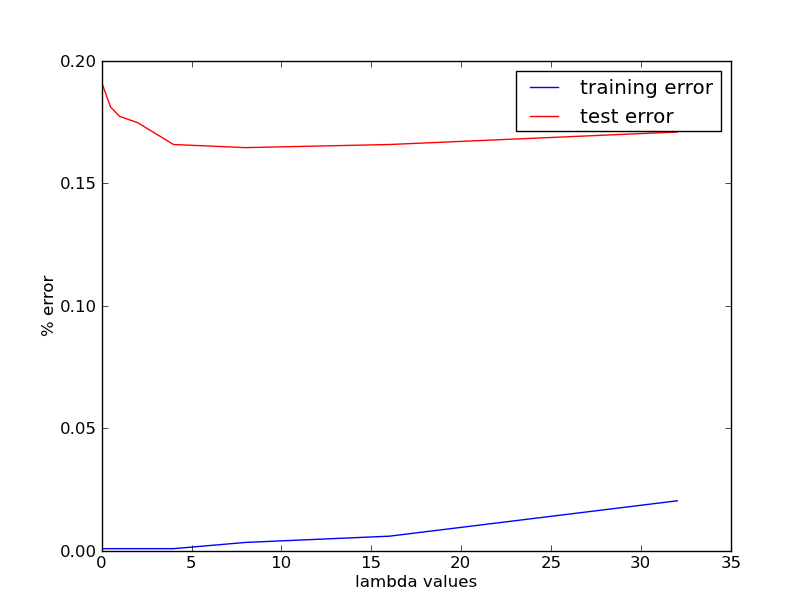
\includegraphics[width=6in]{images/wu6_megam.png}
    \end{figure}

    \begin{figure}
	    \caption{Plot of FastDT error rate with various maxdepths}
	    \label{fig:fastdt}
	    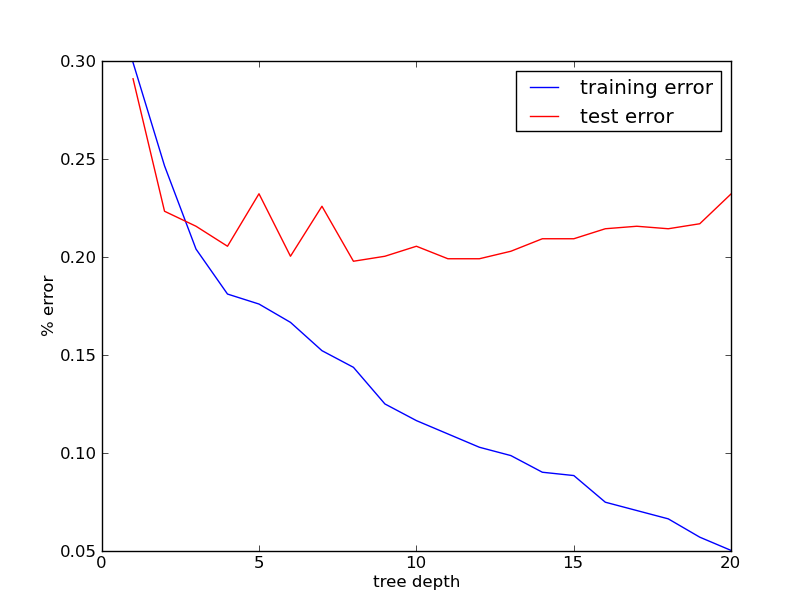
\includegraphics[width=6in]{images/wu6_fastdt.png}
    \end{figure}

    \begin{figure}
	    \caption{Plot of libsvm error rate with various lambda values}
	    \label{fig:libsvm}
	    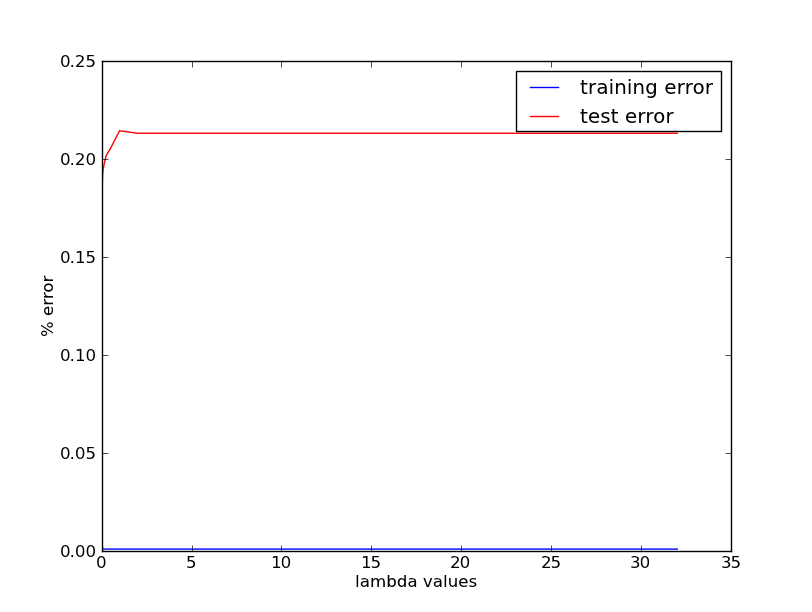
\includegraphics[width=6in]{images/wu6_libsvm.png}
    \end{figure}


\section{WU7}
All three of the algorithms gets an error rate of $7\%$ on the digit recognition using the default values provided in the project description. For the text categorization task, megam performs the best using the default values, with an error rate of $17.7\%$

WHY!?!??!?!?


